\documentclass{beamer}

\usepackage{graphicx} % Required for including images
\graphicspath{{Figures/}}

\usepackage[font=small]{caption}

%Information to be included in the title page:
\title{Rain attenuation of 58GHz radio signal}
\author{Qianhao Zhang}

\begin{document}

\frame{\titlepage}

\begin{frame}
\frametitle{Introduction}
From 8 to 14 week I worked for Space technology laboratory supervised by Dr. László Csurgai-Horváth.
Our project is to measure how rainfull effects the propagation of a 58Ghz radio signal.
\end{frame}

\begin{frame}
\frametitle{Why 58GHz?}

\begin{figure}[h!]
    \centering
    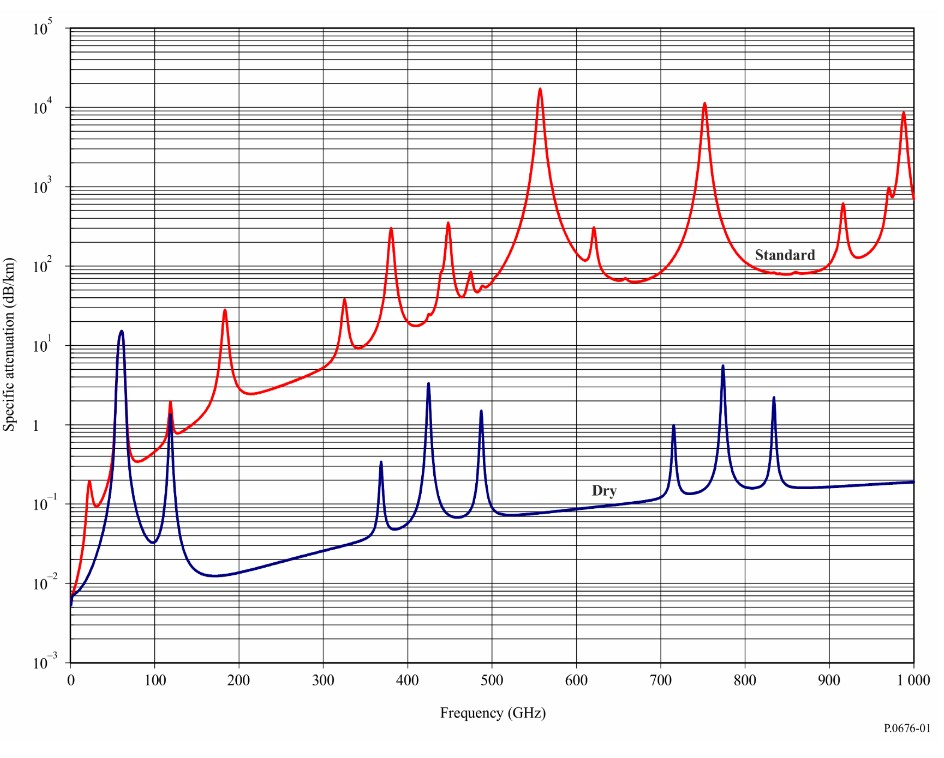
\includegraphics[width=0.9\linewidth]{oxygen.jpg}
    \caption{Atmospheric attenuation}
    \label{fig:Atmospheric attenuation}
\end{figure}
    
\end{frame}

\begin{frame}
\frametitle{Why 58GHz?}
Around this frequency
signal propagation is effected by oxygen molecule in the air. This phenomenon is 
called oxygen attenuation. Because such phenomenon, signal can not propagate for long distance.
\end{frame}

\begin{frame}
    \frametitle{Frequency reuse}
    
    \begin{figure}[h!]
        \centering
        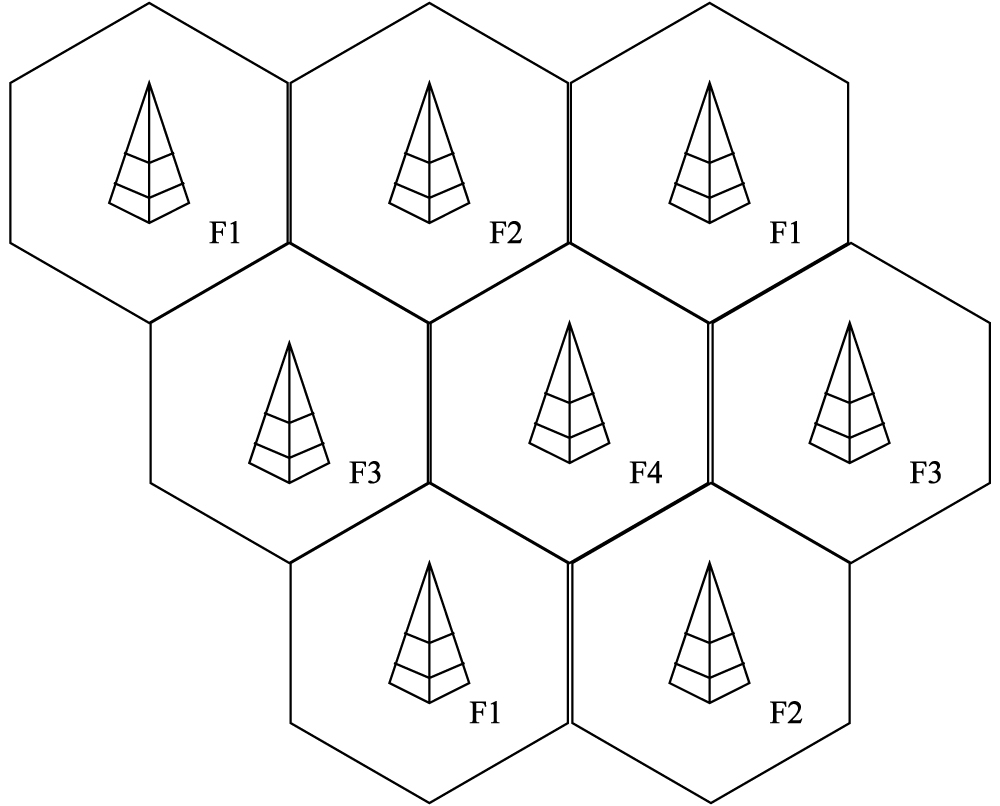
\includegraphics[width=0.9\linewidth]{Frequency_reuse.jpg}
        \caption{Cellular Network}
        \label{fig:Cellular Network}
    \end{figure}
\end{frame}

\begin{frame}{Measurement setup}
    Two outdoor units are installed on the roof of both building V1 and building E. 
    A computer connected to an indoor unit is logging the signal level every 10 second.

    \begin{figure}[h!]
        \centering
        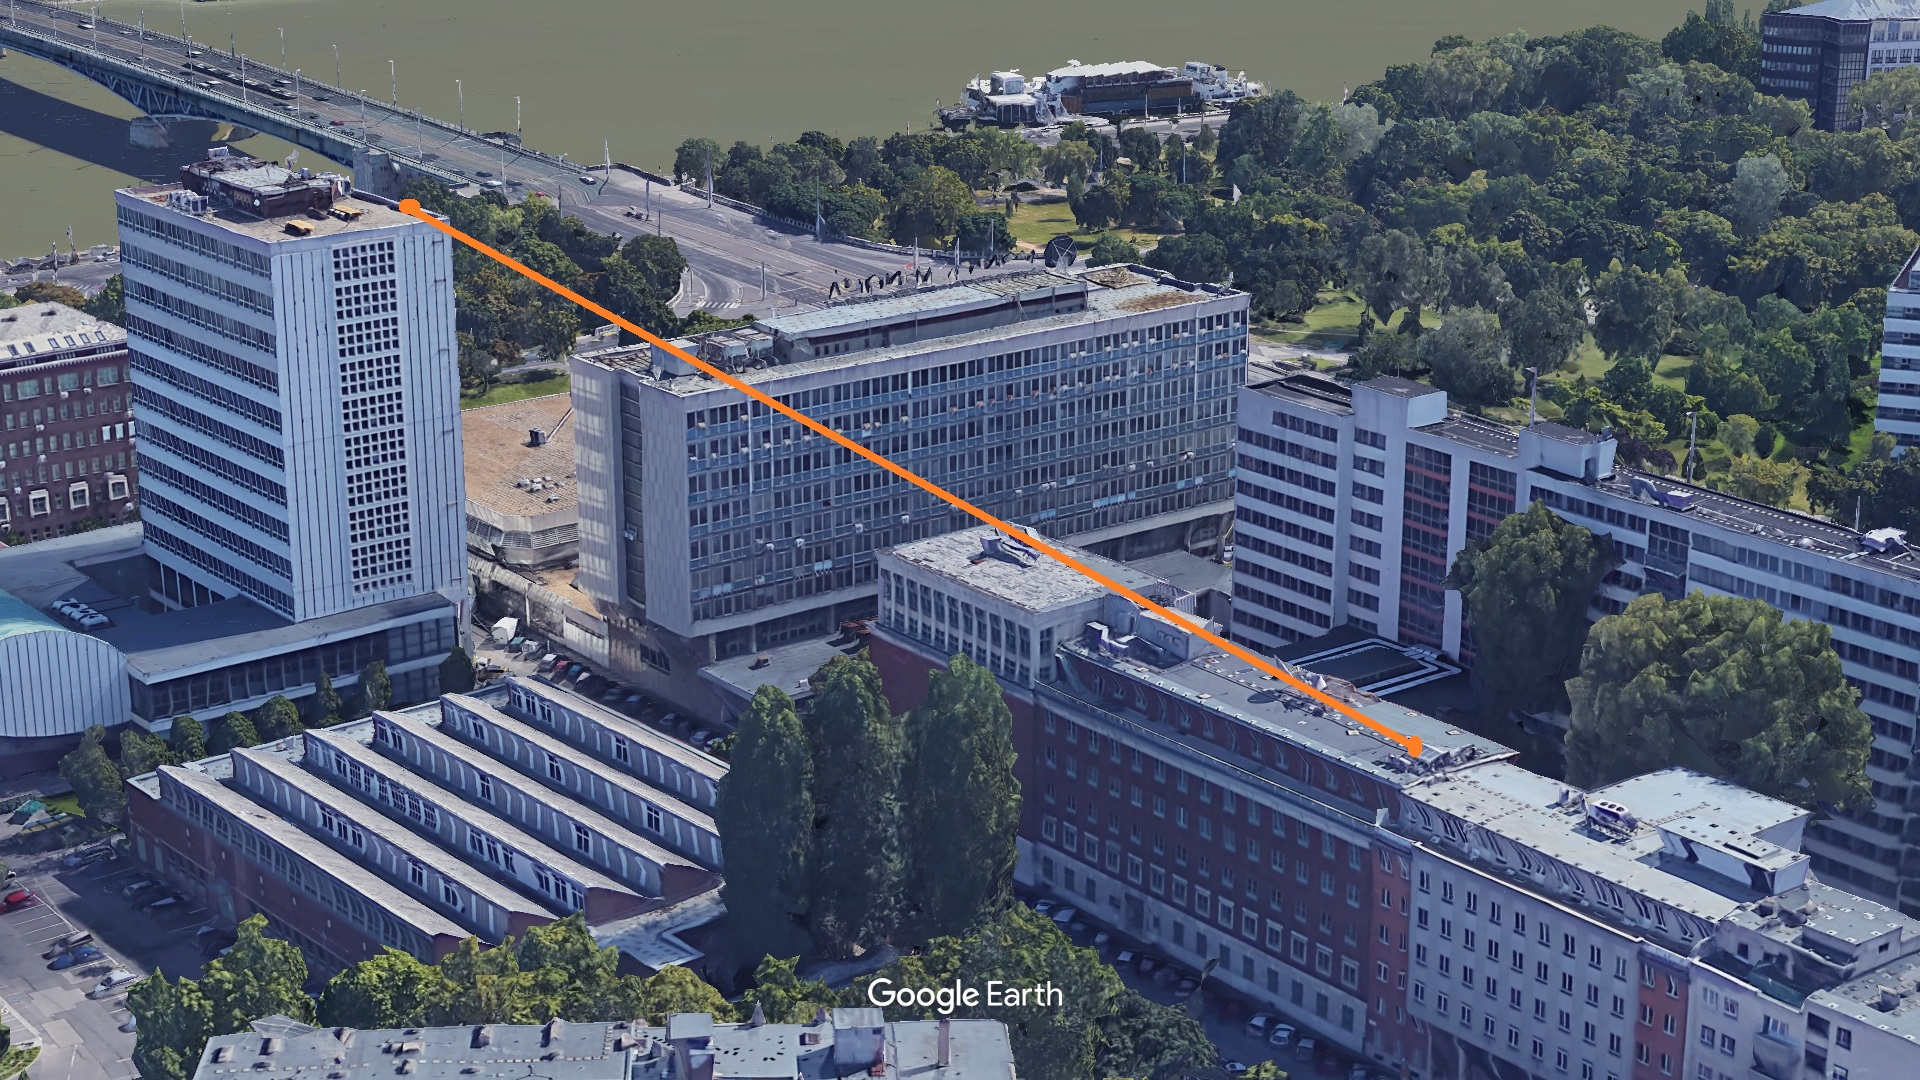
\includegraphics[width=0.9\linewidth]{Google_earth.jpeg}
        \label{fig:google earth}
    \end{figure}
\end{frame}

\begin{frame}{Data processing}
    All measurement data are stored in Oracle Cloud database. I made a python application
    for collecting and uploading the data to the cloud. And a webapp which can make data visualisation 
    within a given time range.

    Webapp: \url{http://152.70.177.227:8080/}
    
\end{frame}

\end{document}